% !TeX program = xelatex
% 插入片段，不含 documentclass、chapter 或 section。
% 將 figsrc/ch02 三張圖片上傳至學姐 Overleaf 專案的同名路徑。

% 放在 2.3.2 介紹場景配置的段落後。
如\cref{fig:isaac_indoor_scene_example}所示，本研究於 Isaac Sim 建立室內模擬場景，配置房間、家具、可動機構及障礙物，作為導航與操作方法的測試環境。
\begin{figure}[htbp]
    \centering
    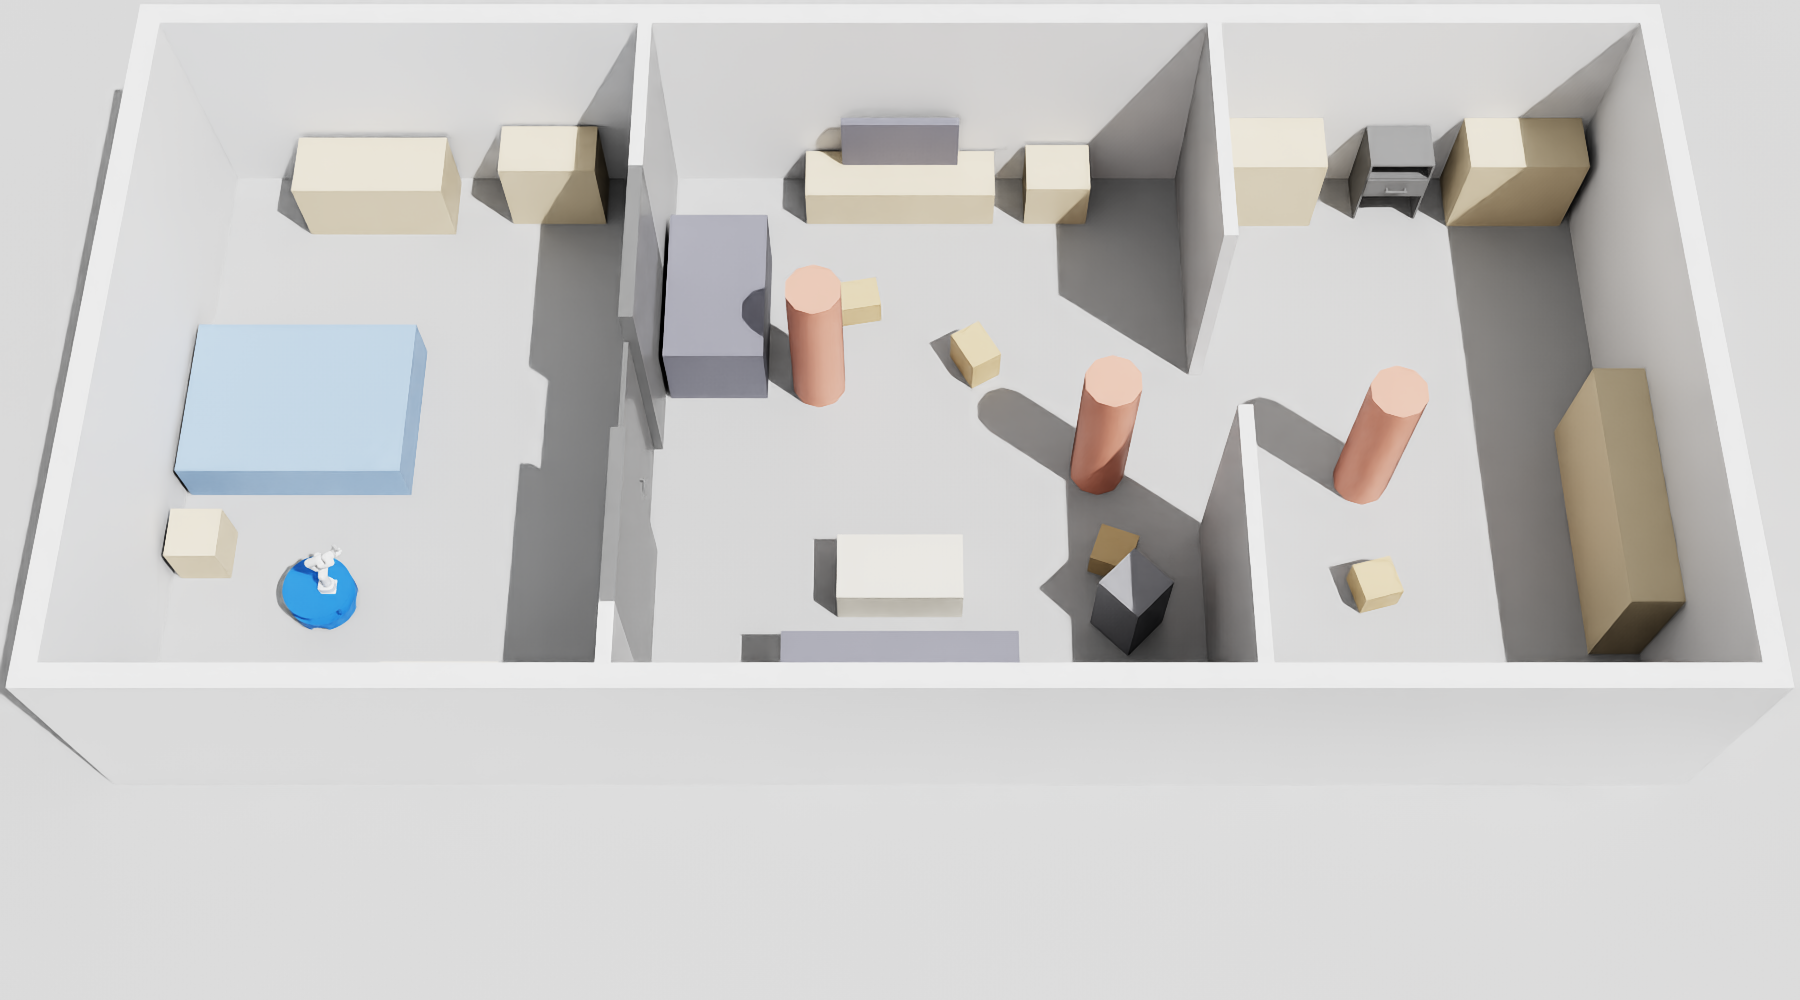
\includegraphics[width=0.95\textwidth]{figsrc/ch02/isaac_indoor_scene_example.png}
    \caption{Isaac Sim 室內模擬場景建置示例}
    \label{fig:isaac_indoor_scene_example}
\end{figure}

% 放在 2.4 節導言後，2.4.1 標題前。
\cref{fig:visual_grasping_workflow}以既有瓶子抓取案例說明視覺資訊與運動控制之間的關係：由影像取得目標遮罩，再結合深度資訊建立三維操作目標，供底盤與手臂協同控制使用。
\begin{figure}[htbp]
    \centering
    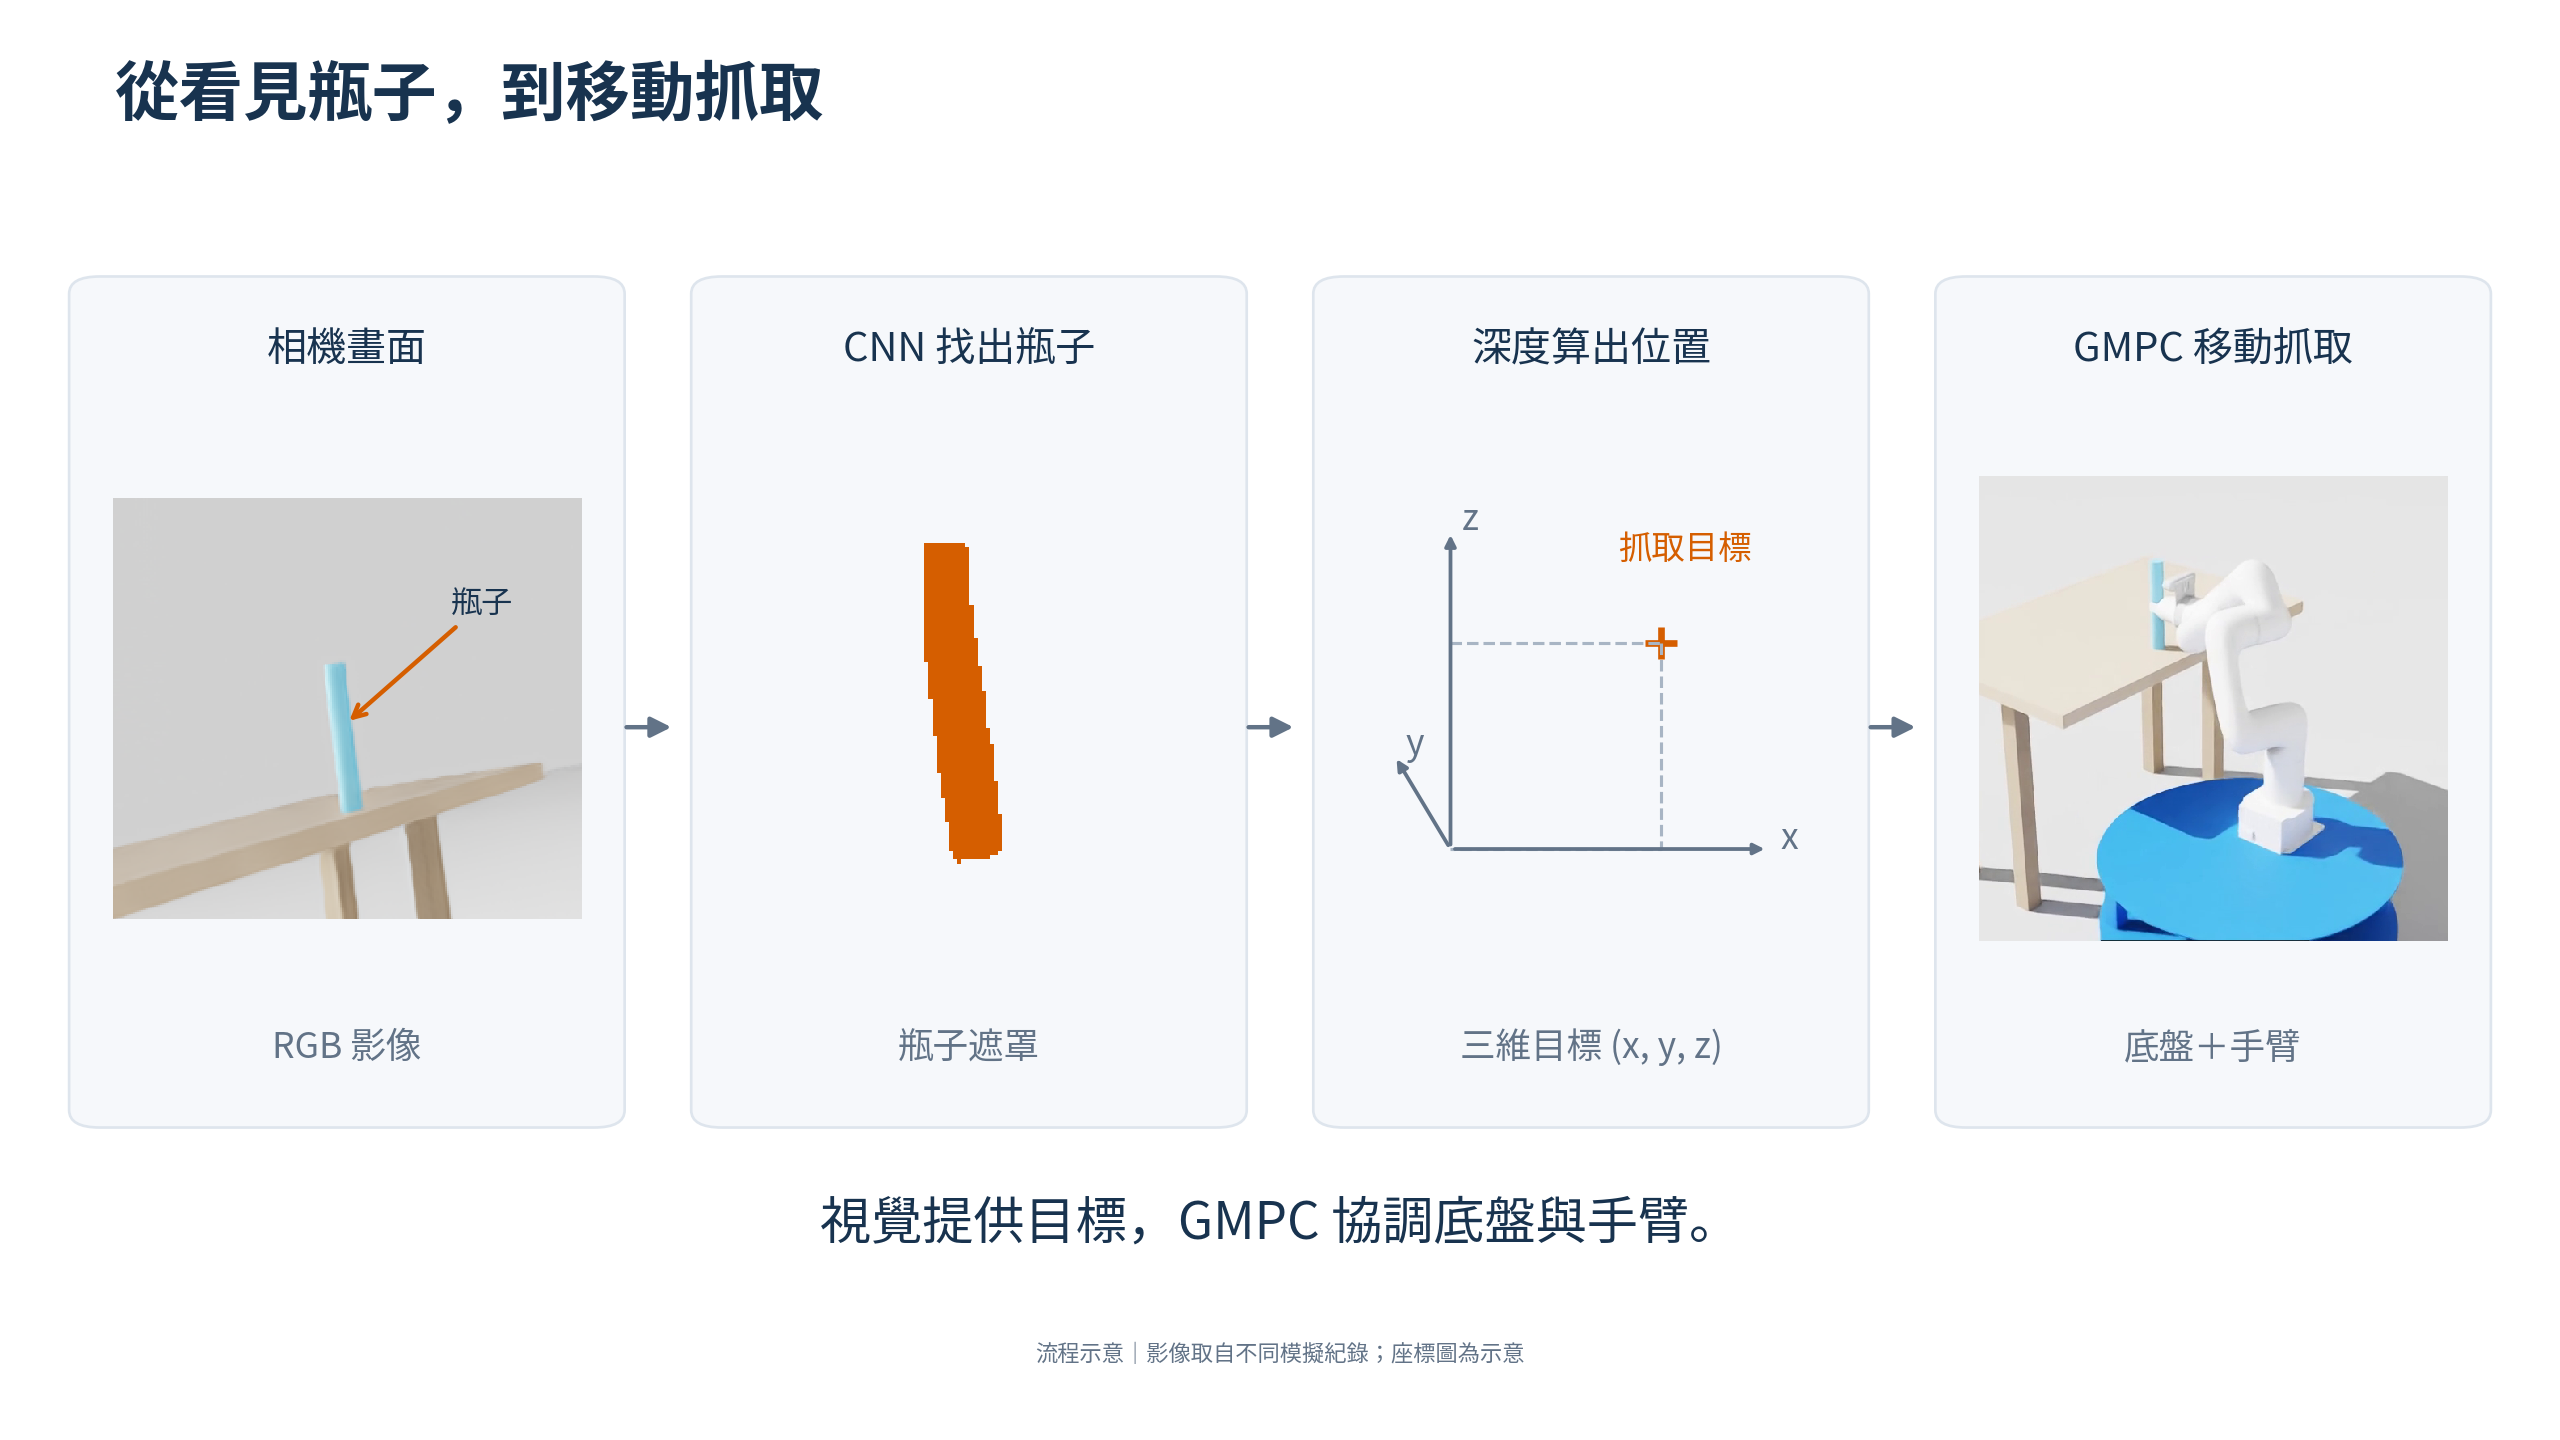
\includegraphics[width=0.98\textwidth]{figsrc/ch02/visual_grasping_workflow.png}
    \caption{視覺導引移動抓取之流程示意；影像取自不同既有模擬紀錄，三維座標為示意}
    \label{fig:visual_grasping_workflow}
\end{figure}

% 放在 2.4.2 介紹影像與深度定位的段落後。
\cref{fig:visual_segmentation_example}呈現既有瓶子辨識案例的原始影像與實例分割結果。偵測框與預測遮罩提供影像中的目標區域，後續再結合深度資料與座標轉換取得三維目標資訊。
\begin{figure}[htbp]
    \centering
    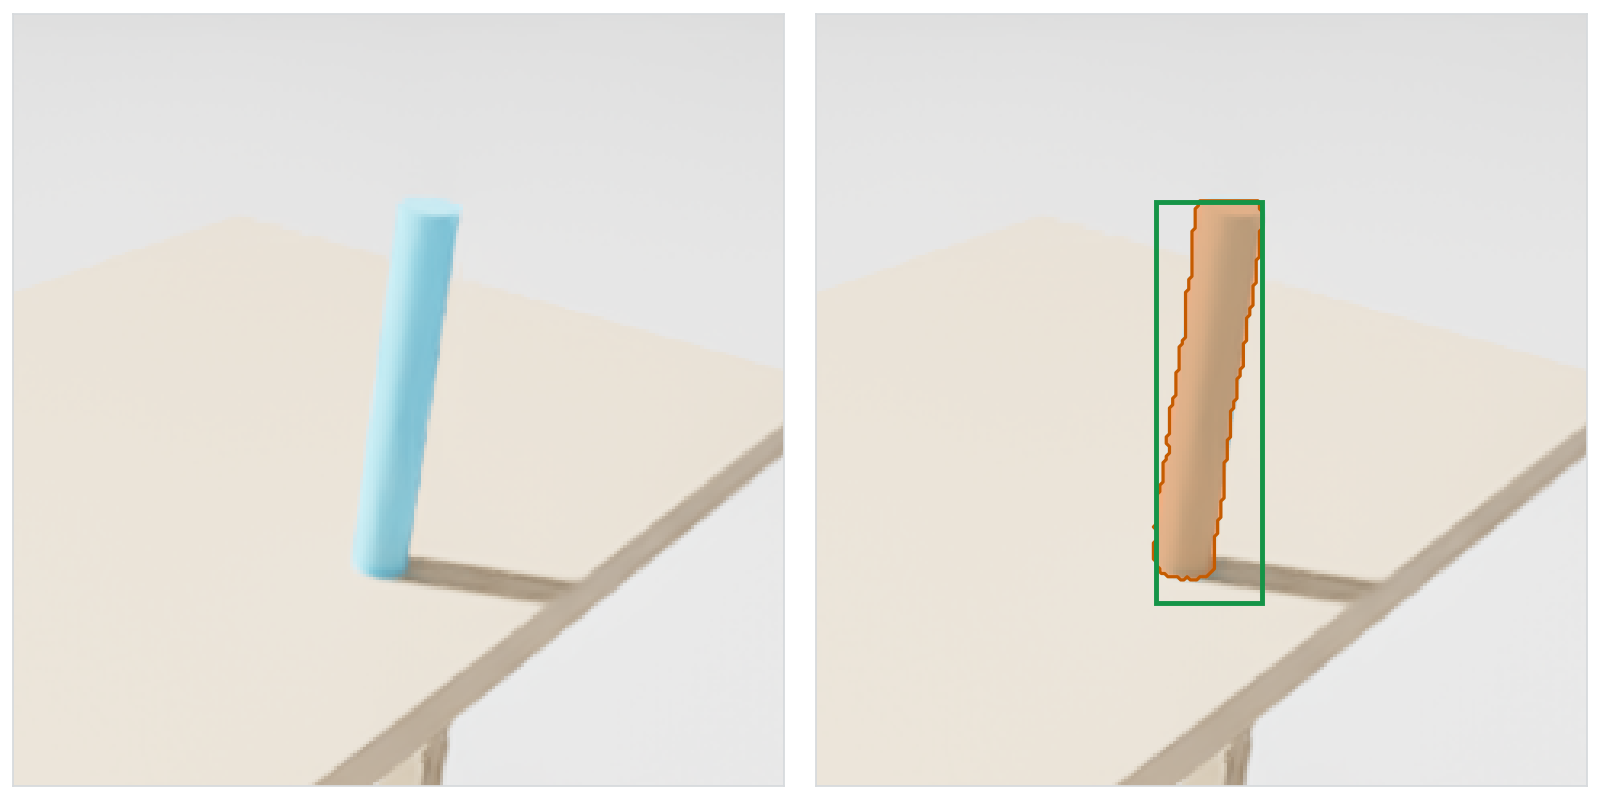
\includegraphics[width=0.90\textwidth]{figsrc/ch02/visual_segmentation_example.png}
    \caption{目標物原始影像與實例分割結果：左圖為原始影像，右圖為偵測框與預測遮罩}
    \label{fig:visual_segmentation_example}
\end{figure}
